\documentclass{article}%
\usepackage[T1]{fontenc}%
\usepackage[utf8]{inputenc}%
\usepackage{lmodern}%
\usepackage{textcomp}%
\usepackage{lastpage}%
\usepackage{authblk}%
\usepackage{graphicx}%
%
\title{JMJD6 is a driver of cellular proliferation and motility and a marker of poor prognosis in breast cancer}%
\author{Kyle Martinez}%
\affil{Department of Gastroenterology, Justus Liebig University, Giessen, Germany}%
\date{01{-}01{-}2013}%
%
\begin{document}%
\normalsize%
\maketitle%
\section{Abstract}%
\label{sec:Abstract}%
BOSTON {-} Boston{-}area researchers have engineered a microbe, a type of cell in the human body, that has a highly similar and extensive signaling pattern to cancer cells.\newline%
The human microbe, unmodified in laboratories, is programmed to use activity generated by another cell, an oncogene, when it is stressed for survival to replace it when it runs out of its natural function. This process greatly increases cell migration and invasion. The mechanisms used in the study could result in the capture of the metastatic cancers as populations reach new levels, from which they may escape as their cells may not be able to stay healthy and multiply properly.\newline%
"Our goal was to see if there was any important difference between a type of cell from cancer and a type of cell from healthy people that would change the cancer cell from a few dozen unfound cells to 50,000 and so on," said a senior author of the study, Sylvain Claude Cul, MD, PhD, a research scientist at Massachusetts General Hospital. "In that respect, what we found is that the selected new cells, though superior to the ones that had been present for generations, produced different results."\newline%
The research team developed the ability to produce a high{-}contrastest microscopy{-}based structure on an oncogene called gp120, which stimulates cell migration and migration into the tumor, hence creating cellular invasion (a target in cancer and in other diseases). In the study, the investigators demonstrated how the monoclonal antibody UT125 binds to and destroys the oncogene, triggering a cellular migration and invasion pathway. They showed that the cell hijacks a mutated version of this particular genes, hence creating a different cell and causing an invasion of the tumor cell.\newline%
HIF1a represents one of the most important pro{-}cancer cells. It is also known to stimulate many other cell types including immune cells such as the anti{-}HIV virus.\newline%
The researchers then optimized the design of the UT125 antibody and added another type of tumor cell, HIF1B, which interacts with gp120 and is primed to attack other tumor cells. These cells are then destroyed in the study.\newline%
Most commonly associated with cancers such as breast cancer, prostate cancer and colon cancer, HIF1a is on the cusp of metastasis and becoming the primary tumor. HIF1B is a cell receptor receptor, also in this population, that promotes the growth of the active tumors and produces a receptor on tumor cells that makes them move and invade the circulating cancer cells.\newline%
"Our two newly shown cells were the ones that the research team chose to manipulate to invade healthy cells," Cul said. "Our limitation, so far, has been to isolate them, because cells need to be cultured using these cells for anti{-}cancer drug resistance to develop."\newline%
The process involved sending millions of sets of M. hifera, an intercellular protein that is ubiquitous in the human body, to the antibody. The antibody can only produce group A+HIF1A (the right cell) in order to be translated into group B+HIF1B (the favored receptor for Oncogene), a subset of the cell.\newline%
To translate these two sets of cells together into a non{-}targeted cell, the researchers developed a function of the specific type of mAb.\newline%
This work is the first to identify a master mAb.

%
\subsection{Image Analysis}%
\label{subsec:ImageAnalysis}%


\begin{figure}[h!]%
\centering%
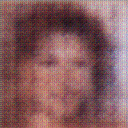
\includegraphics[width=150px]{500_fake_images/samples_5_105.png}%
\caption{A Man With A Beard Wearing A Tie}%
\end{figure}

%
\end{document}